\chapter{Estabilidade}
\label{estabilidade}


\section{Forças Atuantes em Voo}

Para complementar a análise de estabilidade, apresentam-se a seguir duas representações
das forças atuantes sobre a aeronave em voo: um diagrama simplificado, destacando as
forças principais de sustentação, peso, tração e arrasto, e um diagrama complementar
que ilustra como essas forças se distribuem ao longo do comprimento da fuselagem.

\begin{figure}[H]
    \centering
    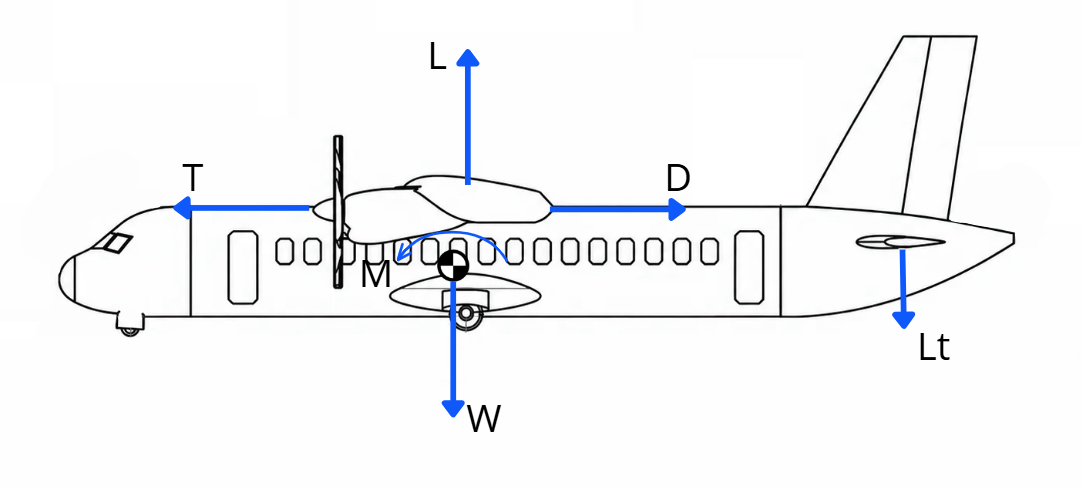
\includegraphics[width=0.92\textwidth]{Images-3-ProjetoDetalhado/CargaPontual.png}
    \caption{Representação simplificada das forças em voo.}
    \label{forcas_em_voo}
\end{figure}

\begin{figure}[H]
    \centering
    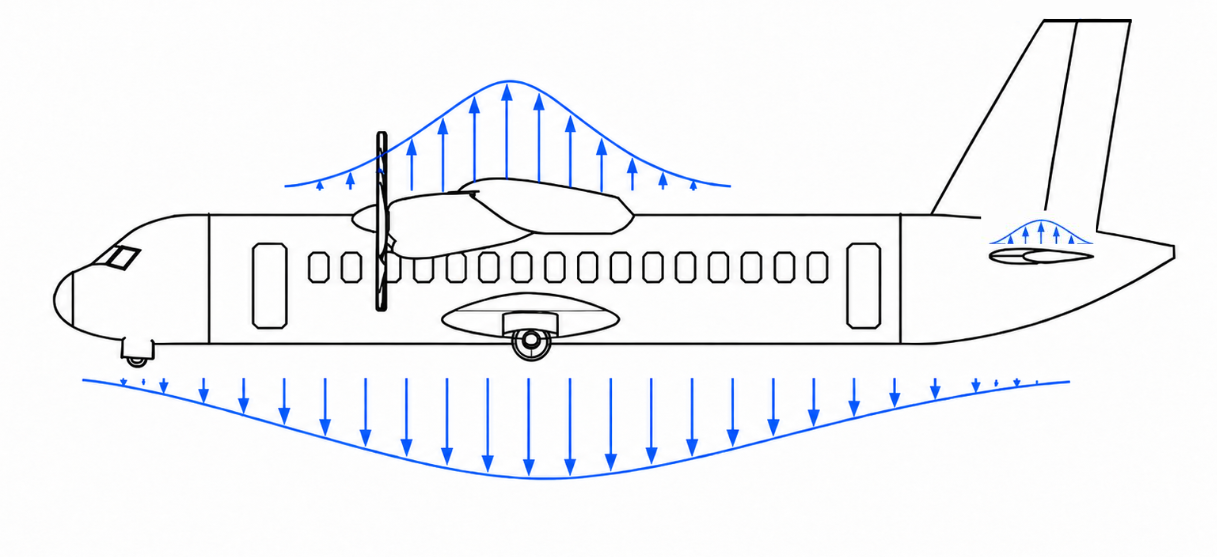
\includegraphics[width=0.92\textwidth]{Images-3-ProjetoDetalhado/CargaDistribuida.png}
    \caption{Representação simplificada das forças distribuídas ao longo da fuselagem.}
    \label{forca_distribuida}
\end{figure}




\section{Análise Preliminar da Estabilidade Longitudinal}

Com a determinação do envelope do centro de gravidade, foi feita uma análise inicial da estabilidade longitudinal da aeronave.



Para isso foi necessário obter as derivadas de estabilidade em torno de uma condição de equilíbrio. Utilizou-se novamente o software AVL para a obtenção desses parâmetros para uma condição de trimagem em cruzeiro da aeronave a uma altitude de 20000 ft.

%====================================================================
%  PONTO 2 -- Tabela de derivadas de estabilidade (inserida logo após
%  a apresentação da obtenção das derivadas no AVL)
%====================================================================

As principais derivadas de estabilidade longitudinal obtidas no AVL, para as duas posições extremas do centro de gravidade analisadas (dianteira e traseira), estão reunidas na Tabela~\ref{tab:derivadas_long} (as demais derivadas obtidas estão listadas nos anexos). Todas as derivadas angulares são expressas por radiano, e as derivadas em relação às velocidades angulares ($C_{L_q}$, $C_{m_q}$) foram convertidas da forma adimensional a partir da expressão ($q\bar{c}/2V$). A posição do centro de gravidade é dada em fração da corda média aerodinâmica ($h_{CG}$), medida a partir do bordo de ataque da CMA, e a margem estática (SM) foi calculada por $\text{SM} = -C_{m_\alpha}/C_{L_\alpha}$, definição equivalente a $\text{SM} = X_{np}/\bar{c} - h_{CG}$ desde que $X_{np}$ seja referido à mesma origem de $h_{CG}$ (o AVL retorna $X_{np}$ a partir do ponto de referência do arquivo \texttt{.avl}, fixado em $c/4$ da CMA, exigindo a correção de $+0{,}25\bar{c}$ ao compará-lo com $h_{CG}$).

\begin{table}[H]
    \centering
    \caption{Derivadas de estabilidade longitudinal e parâmetros associados para as condições extremas de CG, obtidas no AVL a 20000 ft de altitude.}
    \begin{tabular}{|l|c|c|}
       \hline
       \textbf{Parâmetro} & \textbf{CG dianteiro} & \textbf{CG traseiro} \\
       \hline
       $h_{CG}$ (\%  $\bar{c}$)        & $0{,}179$   & $0{,}459$  \\
       \hline
       Margem estática (SM)              & $0{,}587$   & $0{,}307$  \\
       \hline
       $C_{L_\alpha}$ [rad$^{-1}$]       & $5{,}816$   & $5{,}816$  \\
       \hline
       $C_{L_q}$ [rad$^{-1}$]            & $14{,}907$  & $11{,}649$ \\
       \hline
       $C_{m_\alpha}$ [rad$^{-1}$]       & $-3{,}412$  & $-1{,}783$ \\
       \hline
       $C_{m_q}$ [rad$^{-1}$]            & $-42{,}955$ & $-37{,}783$\\
       \hline
    \end{tabular}
    \label{tab:derivadas_long}
\end{table}

Antes da análise modal, verificou-se a coerência física dos sinais das derivadas dominantes em arfagem. Em ambas as condições de CG, $C_{m_\alpha} < 0$ confirma estabilidade estática longitudinal (com margem estática positiva em todo o envelope), e $C_{m_q} < 0$ confirma amortecimento positivo em arfagem. Como esperado, a rigidez estática $C_{m_\alpha}$ e a margem estática são maiores na condição de CG dianteiro, tornando a aeronave mais estável (porém menos manobrável) nessa configuração, e menores na condição traseira, que representa o caso crítico de estabilidade do envelope.

Por fim, com o fim de simplificação de análise, foi feito desacoplamento do movimento longitudinal com o látero-direcional. Dessa forma, as variáveis de estado $\vec{x}_{long}$ e entradas $\vec{u}_{long}$ que descrevem o movimento são:

\begin{equation}
    \vec{x} = \begin{bmatrix} V \\ \alpha \\ \theta \\ q \\ h   \end{bmatrix} \qquad \vec{u} = \begin{bmatrix}
        \eta \\ \delta_t \\
    \end{bmatrix}
\end{equation}

Dessa forma, o sistema dinâmico linearizado pode ser descrito da forma:

\begin{equation}
\dot{\vec{x}} = A_{long} \ \vec{x} + B_{long} \ \vec{u}
\end{equation}

Onde matrizes $A_{long}$ e $B_{long}$ são obtidas a partir dos autovalores do sistema de equações diferencias, que também podem ser encontradas no apêndice.

Para fins de auxilio de cálculo, foi utilizado o MATLAB para a obtenção das matrizes e, consequentemente, dos modos longitudinais e seus polos. Os polos podem ser observados na Fig. \ref{polos}. O movimento longitudinal se apresentou ser dinamicamente estável em todo o intervalo do CG.

%====================================================================
%  PONTO 3 -- Excitação por doublet (inserida logo após a descrição do
%  modelo Simulink e do doublet aplicado)
%====================================================================

Para a simulação, foi feito um modelo dinâmico da aeronave no aplicativo do SIMULINK. Os resultados para a simulação podem ser encontrados no anexo.

\subsection{Dados de Massa e Inércia Empregados}

%====================================================================
%  PONTO 6 -- Dados de massa e inércia / aproximação dos momentos de
%  inércia
%====================================================================

A linearização e a simulação dinâmica exigem, além das derivadas aerodinâmicas, os dados de massa e do tensor de inércia da aeronave. A massa adotada corresponde ao peso máximo de decolagem (MTOW) de $22\,680$~kg. Como a aeronave possui plano de simetria longitudinal ($XZ$), os produtos de inércia $I_{xy}$ e $I_{yz}$ foram considerados nulos, restando os momentos principais $I_{xx}$, $I_{yy}$ e $I_{zz}$ (e, eventualmente, $I_{xz}$).

Na fase atual do projeto, ainda não se dispõe de uma distribuição detalhada de massa da estrutura e dos sistemas que permita o cálculo direto do tensor de inércia por integração. Por esse motivo, os momentos de inércia foram estimados pelo método dos raios de giração, abordagem usual em projeto preliminar, na qual cada momento de inércia é escrito em função da massa da aeronave, de uma dimensão característica e de um raio de giração adimensional $R$, conforme:

\begin{equation}
    I_{xx} = \frac{b^2 \, m \, R_x^2}{4}, \qquad
    I_{yy} = \frac{l_f^2 \, m \, R_y^2}{4}, \qquad
    I_{zz} = \frac{(b + l_f)^2 \, m \, R_z^2}{4}
    \label{eq:inercia_giracao}
\end{equation}

onde $m$ é a massa da aeronave, $b$ a envergadura, $l_f$ o comprimento da fuselagem, e $R_x$, $R_y$ e $R_z$ os raios de giração adimensionais associados, respectivamente, aos eixos de rolamento, arfagem e guinada. A lógica física por trás de cada dimensão característica reflete a distribuição predominante de massa em cada eixo: o momento de inércia em rolamento ($I_{xx}$) é dominado pela distribuição ao longo da envergadura $b$; o momento em arfagem ($I_{yy}$) pela distribuição ao longo do comprimento da fuselagem $l_f$; e o momento em guinada ($I_{zz}$), por envolver simultaneamente a distribuição em ambas as direções, é associado a uma dimensão combinada $(b + l_f)$. Os raios de giração adimensionais foram adotados a partir de valores típicos tabelados para aeronaves de mesma categoria.

Os valores resultantes empregados na análise estão reunidos na Tabela~\ref{tab:inercia}.

\begin{table}[H]
    \centering
    \caption{Massa e momentos de inércia estimados da aeronave.}
    \begin{tabular}{|l|c|}
       \hline
       \textbf{Parâmetro} & \textbf{Valor} \\
       \hline
       Massa (MTOW)            & $22\,680$ kg \\
       \hline
       $I_{xx}$                & $5{,}32 \times 10^{5}$ kg$\cdot$m$^2$ \\
       \hline
       $I_{yy}$                & $3{,}22 \times 10^{5}$ kg$\cdot$m$^2$ \\
       \hline
       $I_{zz}$                & $3{,}26 \times 10^{6}$ kg$\cdot$m$^2$ \\
       \hline
       $I_{xy} = I_{xz} = I_{yz}$ & $0$ \\
       \hline
    \end{tabular}
    \label{tab:inercia}
\end{table}

Cabe ressaltar que essa estimativa, embora adequada para uma análise preliminar de estabilidade, carrega incerteza significativa, uma vez que depende dos raios de giração adotados de referências externas e não da distribuição real de massa da aeronave em projeto. Os momentos de inércia influenciam diretamente o amortecimento e a frequência dos modos dinâmicos (em especial o curto período, fortemente dependente de $I_{yy}$), de modo que esses valores deverão ser refinados em fases posteriores do projeto, à medida que a distribuição de massa estrutural e de sistemas for detalhada.


\subsection{Excitação dos Modos por Doublet}

A excitação dos modos longitudinais foi feita por meio de um \textit{doublet} que consiste em um pulso de deflexão positiva imediatamente seguido por um pulso de deflexão negativa de mesma amplitude, retornando ao valor de trimagem ao final. Essa forma de entrada concentra a energia da excitação em torno de uma faixa estreita de frequência, sendo particularmente adequada para excitar predominantemente o modo de interesse.

A amplitude foi mantida pequena ($1^\circ$ de deflexão) de modo a preservar a validade da hipótese de pequenas perturbações, sobre a qual o modelo linearizado se fundamenta. A largura de cada pulso foi dimensionada de forma a ser da ordem da metade do período do modo de curto período, concentrando assim a excitação na sua frequência natural; o modo de longo período (fugóide), por possuir período muito mais elevado, é excitado de forma secundária pela perturbação inicial e observado na resposta livre subsequente, após o decaimento do transiente de curto período. Vale observar que, por ser uma entrada simétrica que retorna ao trim, o \textit{doublet} pouco altera a velocidade de equilíbrio, característica desejável para a observação do curto período, no qual a velocidade permanece aproximadamente constante.

\begin{figure}[H]
    \centering
    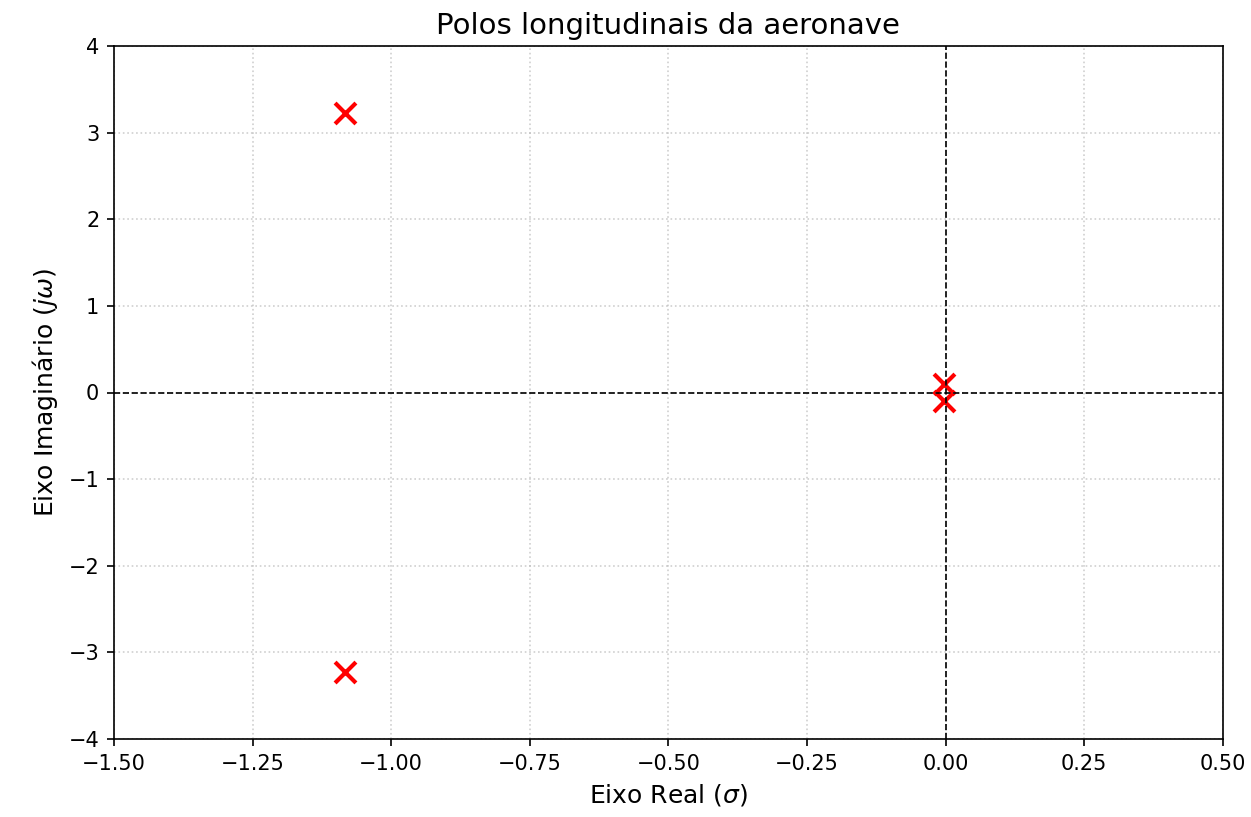
\includegraphics[width=0.5\linewidth]{Polos_projetos.png}
    \caption{Polos para o movimento longitudinal da aeronave.}
    \label{polos}
\end{figure}

\begin{figure}[H]
    \centering
    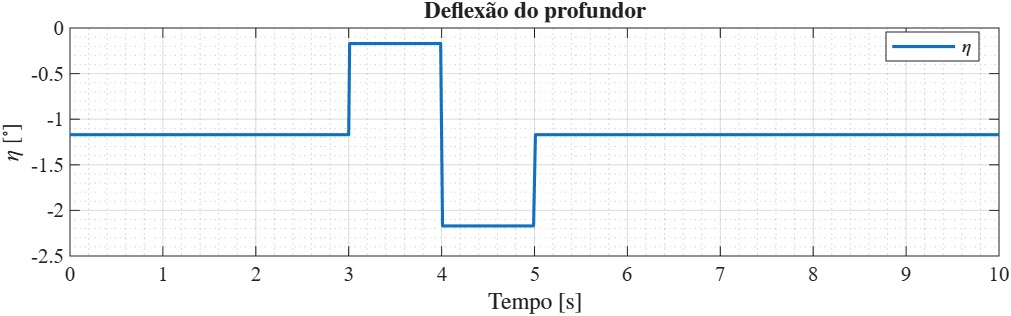
\includegraphics[width=0.5\linewidth]{images/doublet_eta.jpeg}
    \caption{Doublet aplicado no profundor}
    \label{doublet}
\end{figure}


\subsection{Modo Curto Período}

O modo curto período da aeronave tem as seguintes propriedades:

\begin{table}[H]
    \centering
    \caption{Características do curto período.}
    \begin{tabular}{|c|c|}
       \hline
       Polos  & $-1,0835 \pm 3,2287i$ \\
       \hline
       Frequência natural ($\omega_n$) & $3,4057$ rad/s \\
       \hline
       Taxa de amortecimento ($\zeta_{d}$) & $0,3182$\\
       \hline
       Período ($T$) & $1,9460$ s \\
       \hline
       Tempo de decaimento ($t_{1/2}$) & $0,6397$ s \\
       \hline
       Tempo de acomodação 2\% ($t_{s}$) & $3,6916$ s\\
       \hline
    \end{tabular}
    \label{curto_periodo}
\end{table}

O curto período da aeronave apresenta uma alta taxa de amortecimento e um pequeno período, o que auxilia a difícil percepção desse modo pelo piloto. O valor de $\zeta_d$ para o curto período está dentro do previsto na norma militar americana MIL-F-8785C para aeronaves do tipo. Nas Figuras \ref{curto_tras} e \ref{curto_dian} pode ser observado, para as condições traseira e dianteira do CG, a evolução no curto período para os ângulos $\alpha$, $\theta$ e $\gamma$. Demais gráficos podem ser encontrados no anexo.


\begin{figure}[H]
    \centering
    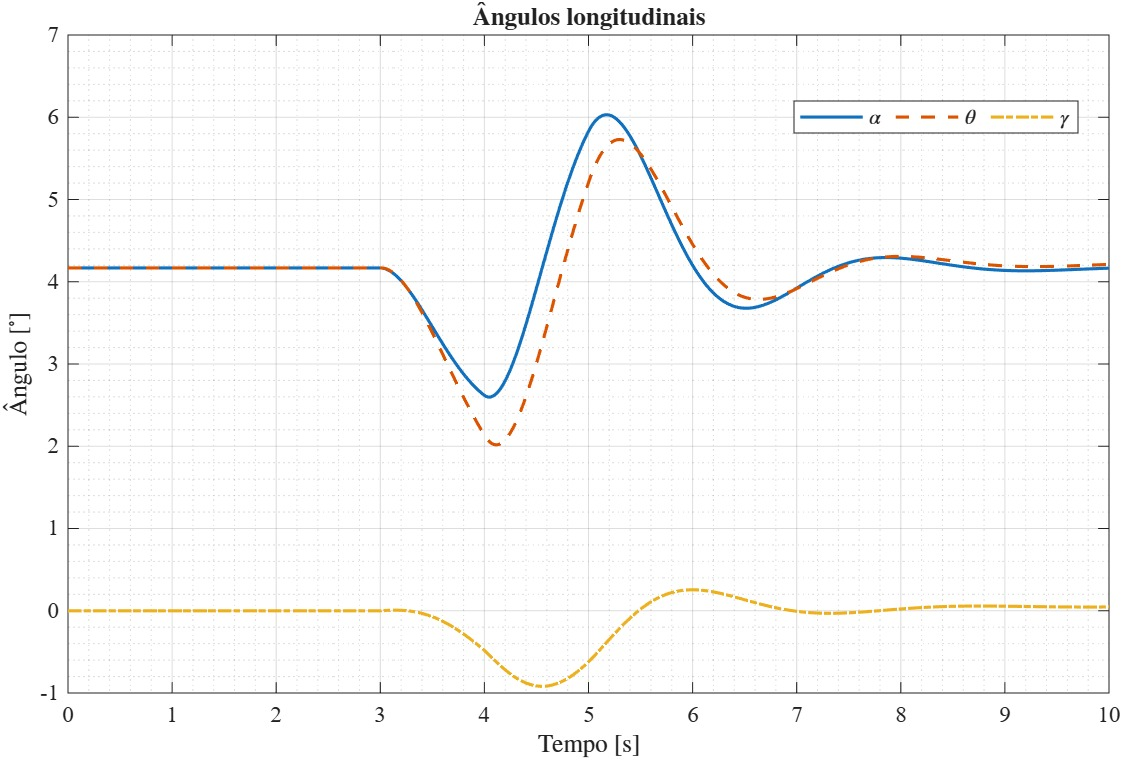
\includegraphics[width=\textwidth]{images/Imagem - desempenho/angulos_curto_CG_traseiro.jpeg}
    \caption{Condição de CG traseiro para o curto período.}
    \label{curto_tras}
\end{figure}

\begin{figure}[H]
    \centering
    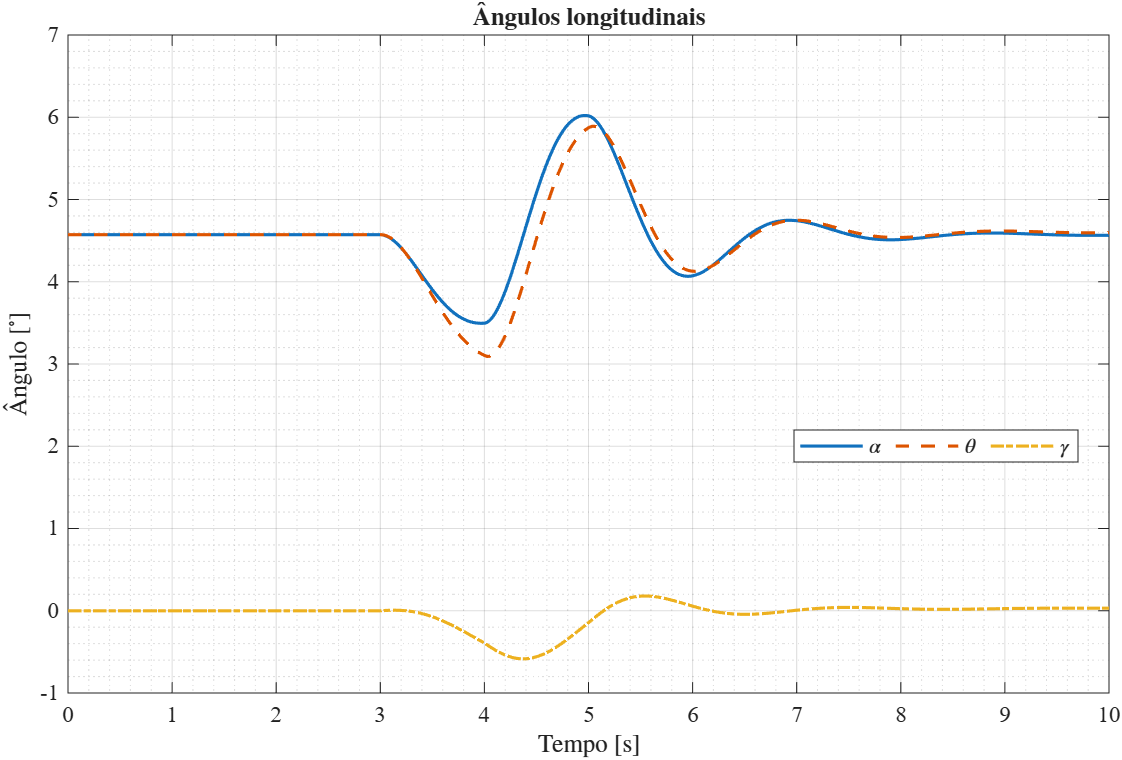
\includegraphics[width=\textwidth]{images/Imagem - desempenho/angulos_CG_dianteiro.png}
    \caption{Condição de CG dianteiro para o curto período.}
    \label{curto_dian}
\end{figure}






\subsection{Modo Longo Período}

%Dados fugóide

O modo longo período ou fugóide da aeronave tem as seguintes propriedades:

\begin{table}[H]
    \centering
    \caption{Características do longo período.}
    \begin{tabular}{|c|c|}
       \hline
       Polos  & $-0.0030 \pm 0.1018i$ \\
       \hline
       Frequência natural ($\omega_n$) & $0,1018$ rad/s \\
       \hline
       Taxa de amortecimento ($\zeta_{d}$) & $0,0291$\\
       \hline
       Período ($T$) & $61,7479$ s \\
       \hline
       Tempo de decaimento ($t_{1/2}$) & $234$ s \\
       \hline
       Tempo de acomodação 2\% ($t_{s}$) & $1350$ s\\
       \hline
    \end{tabular}
    \label{longo_periodo}
\end{table}

O modo longo período apresenta um amortecimento extremamente baixo (mesmo para os padrões da fugóide), fazendo com que a aeronave oscile muito tempo até retornar a condição de equilíbrio. Entretanto, o período também é de magnitude considerável o que ajuda a não percepção desse movimento, fazendo com que o baixo amortecimento não seja problemático. A aeronave consta dentro das especificações da norma MIL-F-8785C para aeronaves desse tipo. Nas Figuras \ref{longo_tras} e \ref{longo_dian} pode ser observado para ambos limites do CG a resposta da velocidade e altitude ao longo período. Gráficos das demais variáveis estão apresentados no anexo.


\begin{figure}[H]
    \centering
    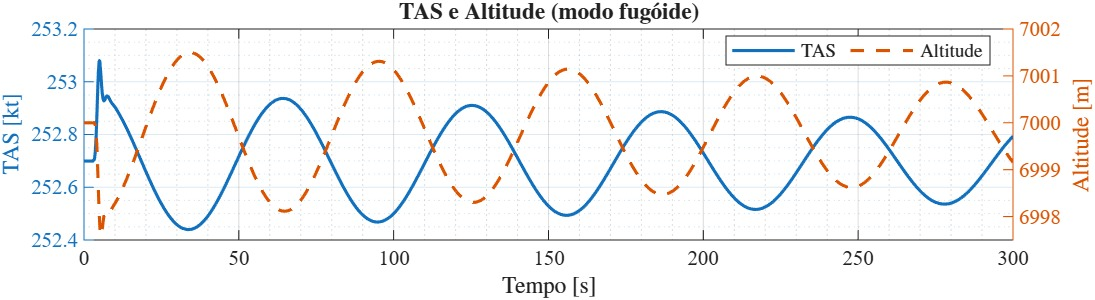
\includegraphics[width=\textwidth]{images/h_longo_CG_trazeiro.jpeg}
    \caption{Condição de CG traseiro para o longo período.}
    \label{longo_tras}
\end{figure}

\begin{figure}[H]
    \centering
    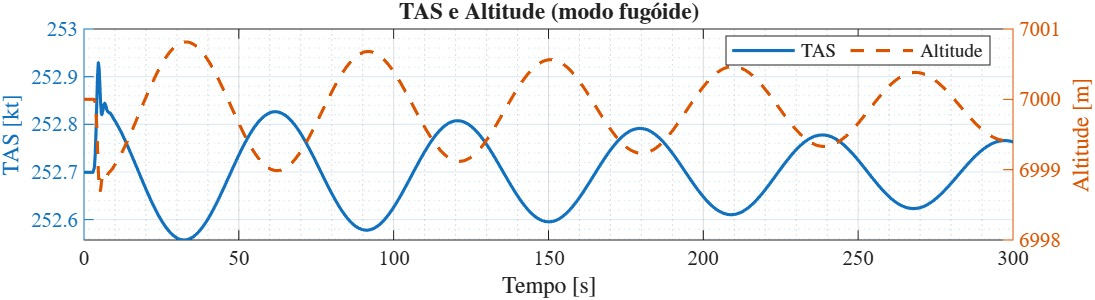
\includegraphics[width=\textwidth]{images/h_longo_CG_dianteiro.jpeg}
    \caption{Condição de CG dianteiro para o longo período.}
    \label{longo_dian}
\end{figure}

%====================================================================
%  PONTO 5 -- Validação cruzada simulação x linearização (inserida
%  após a apresentação dos dois modos, antes das conclusões)
%====================================================================

\subsection{Validação Cruzada entre a Linearização e a Simulação Não-linear}

Os modos longitudinais foram caracterizados por duas vias independentes, que se validam mutuamente. Os valores de frequência natural, amortecimento e período apresentados nas Tabelas~\ref{curto_periodo} e \ref{longo_periodo} foram obtidos analiticamente, a partir dos autovalores da matriz $A_{long}$ resultante da linearização do modelo no ponto de equilíbrio. Esses parâmetros não dependem da integração no tempo, sendo determinados unicamente pelo ponto de trimagem.

Como verificação independente, a resposta temporal obtida na simulação não-linear no SIMULINK foi confrontada com esses valores, obtendo resultados muito próximos da simulação linearizada. A concordância entre as duas abordagens, uma analítica e outra numérica não-linear, confere confiança ao modelo linear empregado e indica que a linearização captura adequadamente a dinâmica longitudinal da aeronave na vizinhança da condição de cruzeiro analisada.



\subsection{Conclusões}

A aeronave é caracterizada como dinamicamente estável em voo de cruzeiro em uma condição de voo reto nivelado, com características dos modos de longo e curto período que se adéquam à norma MIL-F-8785C para seu tipo. Para uma análise mais profunda de qualidade de voo é necessário avaliar a estabilidade látero direcial. Por fim, apesar das normas demonstrarem uma boa ideia sobre a validação das características dos modos longitudinais, uma avaliação completa dos modos longitudinais é feita em partes mais avançadas dor projeto, com dados de testes de modelos e ensaios em voo.


